% !TeX root = ../Template.tex
% 本LaTeX模板的使用示例
\chapter{示例}

%==============================
\section{参考文献引用}

%--------------------------------
\subsection{数字标注}
\noindent
\begin{tabular}{l@{\quad$\Rightarrow$\quad}l}
  \verb|\cite{knuth86a}| & \cite{knuth86a}\\
  \verb|\citet{knuth86a}| & \citet{knuth86a}\\
  \verb|\citet[chap.~2]{knuth86a}| & \citet[chap.~2]{knuth86a}\\[0.5ex]
  \verb|\citep{knuth86a}| & \citep{knuth86a}\\
  \verb|\citep[chap.~2]{knuth86a}| & \citep[chap.~2]{knuth86a}\\
  \verb|\citep[see][]{knuth86a}| & \citep[see][]{knuth86a}\\
  \verb|\citep[see][chap.~2]{knuth86a}| & \citep[see][chap.~2]{knuth86a}\\[0.5ex]
  \verb|\citet*{knuth86a}| & \citet*{knuth86a}\\
  \verb|\citep*{knuth86a}| & \citep*{knuth86a}\\
\end{tabular}
\par\noindent
\begin{tabular}{l@{\quad$\Rightarrow$\quad}l}
  \verb|\citet{knuth86a,tlc2}| & \citet{knuth86a,tlc2}\\
  \verb|\citep{knuth86a,tlc2}| & \citep{knuth86a,tlc2}\\
  \verb|\cite{knuth86a,knuth84}| & \cite{knuth86a,knuth84}\\
  \verb|\upcite{knuth86a,knuth84}| & \upcite{knuth86a,knuth84}\\
  \verb|\citet{knuth86a,knuth84}| & \citet{knuth86a,knuth84}\\
  \verb|\citep{knuth86a,knuth84}| & \citep{knuth86a,knuth84}\\
  \verb|\cite{knuth86a,knuth84,tlc2}| & \cite{knuth86a,knuth84,tlc2}\\
\end{tabular}

%--------------------------------
\subsection{数字标注-上标形式}
\noindent
\begin{tabular}{l@{\quad$\Rightarrow$\quad}l}
  \verb|\upcite{knuth86a}| & \upcite{knuth86a}\\
  \verb|\upcite{knuth86a,knuth84,tlc2}| & \upcite{knuth86a,knuth84,tlc2}\\
\end{tabular}
\par\noindent
实现源码:\verb|\newcommand{\upcite}[1]{\textsuperscript{\cite{#1}}}|。


%--------------------------------
\subsection{著者-出版年制标}
\citestyle{authoryear}
\noindent
\begin{tabular}{l@{\quad$\Rightarrow$\quad}l}
  \verb|\cite{knuth86a}| & \cite{knuth86a}\\
  \verb|\citet{knuth86a}| & \citet{knuth86a}\\
  \verb|\citet[chap.~2]{knuth86a}| & \citet[chap.~2]{knuth86a}\\[0.5ex]
  \verb|\citep{knuth86a}| & \citep{knuth86a}\\
  \verb|\citep[chap.~2]{knuth86a}| & \citep[chap.~2]{knuth86a}\\
  \verb|\citep[see][]{knuth86a}| & \citep[see][]{knuth86a}\\
  \verb|\citep[see][chap.~2]{knuth86a}| & \citep[see][chap.~2]{knuth86a}\\[0.5ex]
  \verb|\citet*{knuth86a}| & \citet*{knuth86a}\\
  \verb|\citep*{knuth86a}| & \citep*{knuth86a}\\
\end{tabular}
\par\noindent
\begin{tabular}{l@{\quad$\Rightarrow$\quad}l}
  \verb|\citet{knuth86a,tlc2}| & \citet{knuth86a,tlc2}\\
  \verb|\citep{knuth86a,tlc2}| & \citep{knuth86a,tlc2}\\
  \verb|\cite{knuth86a,knuth84}| & \cite{knuth86a,knuth84}\\
  \verb|\citet{knuth86a,knuth84}| & \citet{knuth86a,knuth84}\\
  \verb|\citep{knuth86a,knuth84}| & \citep{knuth86a,knuth84}\\
\end{tabular}
\citestyle{numbers}

%--------------------------------
\subsection{其他形式的标注}
\noindent
\begin{tabular}{l@{\quad$\Rightarrow$\quad}l}
  \verb|\citealt{tlc2}| & \citealt{tlc2}\\
  \verb|\citealt*{tlc2}| & \citealt*{tlc2}\\
  \verb|\citealp{tlc2}| & \citealp{tlc2}\\
  \verb|\citealp*{tlc2}| & \citealp*{tlc2}\\
  \verb|\citealp{tlc2,knuth86a}| & \citealp{tlc2,knuth86a}\\
  \verb|\citealp[pg.~32]{tlc2}| & \citealp[pg.~32]{tlc2}\\
  \verb|\citenum{tlc2}| & \citenum{tlc2}\\
  \verb|\citetext{priv.\ comm.}| & \citetext{priv.\ comm.}\\
\end{tabular}

\noindent
\begin{tabular}{l@{\quad$\Rightarrow$\quad}l}
  \verb|\citeauthor{tlc2}| & \citeauthor{tlc2}\\
  \verb|\citeauthor*{tlc2}| & \citeauthor*{tlc2}\\
  \verb|\citeyear{tlc2}| & \citeyear{tlc2}\\
  \verb|\citeyearpar{tlc2}| & \citeyearpar{tlc2}\\
\end{tabular}

\section{浮动体}

\section{算法环境}

模板中使用 \texttt{algorithm2e} 宏包实现算法环境。关于该宏包的具体用法请阅读宏包的官方文档。\\
\centerline{-----------$\downarrow$-----------Space Check-----------$\downarrow$-----------}

\begin{algorithm}[!h]
  %\SetAlgoLined
  %\SetAlgoVlined
  \caption{A How to (plain).}
  \KwData{this text}
  \KwResult{how to write algorithm with \LaTeX2e{} }
  
  initialization\;
  \While{not at end of this document}{
    read current\;
    \eIf{understand}{
      go to next section\;
      current section becomes this one\;
    }{
      go back to the beginning of current section\;
    }
  }
\end{algorithm}

\centerline{-----------$\uparrow$-----------Space Check-----------$\uparrow$-----------}

\RestyleAlgo{ruled}
\begin{algorithm}[!h]
  \caption{A How to (ruled).}
  \KwData{this text}
  \KwResult{how to write algorithm with \LaTeX2e{} }
  
  initialization\;
  \While{not at end of this document}{
    read current\;
    \eIf{understand}{
      go to next section\;
      current section becomes this one\;
    }{
      go back to the beginning of current section\;
    }
  }
\end{algorithm}

\RestyleAlgo{boxed}
\begin{algorithm}[!h]
  \caption{A How to (boxed).}
  \KwData{this text}
  \KwResult{how to write algorithm with \LaTeX2e{} }
  
  initialization\;
  \While{not at end of this document}{
    read current\;
    \eIf{understand}{
      go to next section\;
      current section becomes this one\;
    }{
      go back to the beginning of current section\;
    }
  }
\end{algorithm}

\RestyleAlgo{boxruled}
\begin{algorithm}[!h]
  \caption{A How to (boxruled).}
  \KwData{this text}
  \KwResult{how to write algorithm with \LaTeX2e{} }
  
  initialization\;
  \While{not at end of this document}{
    read current\;
    \eIf{understand}{
      go to next section\;
      current section becomes this one\;
    }{
      go back to the beginning of current section\;
    }
  }
\end{algorithm}

\subsection{三线表}
推荐使用三线表的方式,如表~\ref{tab:exampletable}。\\
\centerline{-----------$\downarrow$-----------Space Check-----------$\downarrow$-----------}

\begin{table}[!h]
  \centering
  \caption{表的标题}
  \label{tab:exampletable}
  \begin{tabular}{p{4cm}p{4cm}}
    \toprule
    \multicolumn{1}{c}{\textbf{操作系统}} & \multicolumn{1}{c}{\textbf{TeX 发行版}} \\
    \midrule
    所有 & TeX Live \\
    macOS & MacTeX \\
    Windows & MikTeX \\
    \bottomrule
  \end{tabular}
\end{table}

\begin{table}[!h]
  \centering
  \caption{让我们看看一个长标题长什么样。还不够长?那我再多写一点。还是不够长?那我再多写一点点。OK,就是长这样的!}
  \label{tab:exampletable}
  \begin{tabular}{p{4cm}p{4cm}}
    \toprule
    \multicolumn{1}{c}{\textbf{操作系统}} & \multicolumn{1}{c}{\textbf{TeX 发行版}} \\
    \midrule
    所有 & TeX Live \\
    macOS & MacTeX \\
    Windows & MikTeX \\
    \bottomrule
  \end{tabular}
\end{table}

\centerline{-----------$\uparrow$-----------Space Check-----------$\uparrow$-----------}

我们在这儿插入一行字;

我们在这儿再插入一行字;

我们在这儿插入一行字;

我们在这儿再插入一行字;

我们在这儿插入一行字;

我们在这儿再插入一行字;

我们在这儿插入一行字;

我们在这儿再插入一行字;

\section{长表格}

超过一页的表格要使用专门的 \texttt{longtable} 环境(表~\ref{tab:longtable})。\\
\centerline{-----------$\downarrow$-----------Space Check-----------$\downarrow$-----------}


\begin{longtable}[h]{ccc}
  % 首页表头
  \caption[长表格演示]{长表格演示}
  \label{tab:longtable}\\
  \toprule
  名称  & 说明 & 备注\\
  \midrule
  \endfirsthead
  % 续页表头
  \caption[]{长表格演示(续)} \\
  \toprule
  名称  & 说明 & 备注 \\
  \midrule
  \endhead
  % 首页表尾
  \hline
  \multicolumn{3}{r}{\small 续下页}
  \endfoot
  % 续页表尾
  \bottomrule
  \endlastfoot
  
  AAAAAAAAAAAA   &   BBBBBBBBBBB   &   CCCCCCCCCCCCCC   \\
  AAAAAAAAAAAA   &   BBBBBBBBBBB   &   CCCCCCCCCCCCCC   \\
  AAAAAAAAAAAA   &   BBBBBBBBBBB   &   CCCCCCCCCCCCCC   \\
  AAAAAAAAAAAA   &   BBBBBBBBBBB   &   CCCCCCCCCCCCCC   \\
  AAAAAAAAAAAA   &   BBBBBBBBBBB   &   CCCCCCCCCCCCCC   \\
  AAAAAAAAAAAA   &   BBBBBBBBBBB   &   CCCCCCCCCCCCCC   \\
  AAAAAAAAAAAA   &   BBBBBBBBBBB   &   CCCCCCCCCCCCCC   \\
  AAAAAAAAAAAA   &   BBBBBBBBBBB   &   CCCCCCCCCCCCCC   \\
  AAAAAAAAAAAA   &   BBBBBBBBBBB   &   CCCCCCCCCCCCCC   \\
  AAAAAAAAAAAA   &   BBBBBBBBBBB   &   CCCCCCCCCCCCCC   \\
  AAAAAAAAAAAA   &   BBBBBBBBBBB   &   CCCCCCCCCCCCCC   \\
  AAAAAAAAAAAA   &   BBBBBBBBBBB   &   CCCCCCCCCCCCCC   \\
  AAAAAAAAAAAA   &   BBBBBBBBBBB   &   CCCCCCCCCCCCCC   \\
  AAAAAAAAAAAA   &   BBBBBBBBBBB   &   CCCCCCCCCCCCCC   \\
  AAAAAAAAAAAA   &   BBBBBBBBBBB   &   CCCCCCCCCCCCCC   \\
  AAAAAAAAAAAA   &   BBBBBBBBBBB   &   CCCCCCCCCCCCCC   \\
  AAAAAAAAAAAA   &   BBBBBBBBBBB   &   CCCCCCCCCCCCCC   \\
  AAAAAAAAAAAA   &   BBBBBBBBBBB   &   CCCCCCCCCCCCCC   \\
  AAAAAAAAAAAA   &   BBBBBBBBBBB   &   CCCCCCCCCCCCCC   \\
  AAAAAAAAAAAA   &   BBBBBBBBBBB   &   CCCCCCCCCCCCCC   \\
  AAAAAAAAAAAA   &   BBBBBBBBBBB   &   CCCCCCCCCCCCCC   \\
  AAAAAAAAAAAA   &   BBBBBBBBBBB   &   CCCCCCCCCCCCCC   \\
  AAAAAAAAAAAA   &   BBBBBBBBBBB   &   CCCCCCCCCCCCCC   \\
  AAAAAAAAAAAA   &   BBBBBBBBBBB   &   CCCCCCCCCCCCCC   \\
  AAAAAAAAAAAA   &   BBBBBBBBBBB   &   CCCCCCCCCCCCCC   \\
  AAAAAAAAAAAA   &   BBBBBBBBBBB   &   CCCCCCCCCCCCCC   \\
  AAAAAAAAAAAA   &   BBBBBBBBBBB   &   CCCCCCCCCCCCCC   \\
  AAAAAAAAAAAA   &   BBBBBBBBBBB   &   CCCCCCCCCCCCCC   \\
  AAAAAAAAAAAA   &   BBBBBBBBBBB   &   CCCCCCCCCCCCCC   \\
  AAAAAAAAAAAA   &   BBBBBBBBBBB   &   CCCCCCCCCCCCCC   \\
  AAAAAAAAAAAA   &   BBBBBBBBBBB   &   CCCCCCCCCCCCCC   \\
  AAAAAAAAAAAA   &   BBBBBBBBBBB   &   CCCCCCCCCCCCCC   \\
  AAAAAAAAAAAA   &   BBBBBBBBBBB   &   CCCCCCCCCCCCCC   \\
  AAAAAAAAAAAA   &   BBBBBBBBBBB   &   CCCCCCCCCCCCCC   \\
  AAAAAAAAAAAA   &   BBBBBBBBBBB   &   CCCCCCCCCCCCCC   \\
  AAAAAAAAAAAA   &   BBBBBBBBBBB   &   CCCCCCCCCCCCCC   \\
  AAAAAAAAAAAA   &   BBBBBBBBBBB   &   CCCCCCCCCCCCCC   \\
  AAAAAAAAAAAA   &   BBBBBBBBBBB   &   CCCCCCCCCCCCCC   \\
  AAAAAAAAAAAA   &   BBBBBBBBBBB   &   CCCCCCCCCCCCCC   \\
  AAAAAAAAAAAA   &   BBBBBBBBBBB   &   CCCCCCCCCCCCCC   \\
  AAAAAAAAAAAA   &   BBBBBBBBBBB   &   CCCCCCCCCCCCCC   \\
  AAAAAAAAAAAA   &   BBBBBBBBBBB   &   CCCCCCCCCCCCCC   \\
  AAAAAAAAAAAA   &   BBBBBBBBBBB   &   CCCCCCCCCCCCCC   \\
  AAAAAAAAAAAA   &   BBBBBBBBBBB   &   CCCCCCCCCCCCCC   \\
  AAAAAAAAAAAA   &   BBBBBBBBBBB   &   CCCCCCCCCCCCCC   \\
  AAAAAAAAAAAA   &   BBBBBBBBBBB   &   CCCCCCCCCCCCCC   \\
  AAAAAAAAAAAA   &   BBBBBBBBBBB   &   CCCCCCCCCCCCCC   \\
  AAAAAAAAAAAA   &   BBBBBBBBBBB   &   CCCCCCCCCCCCCC   \\
  AAAAAAAAAAAA   &   BBBBBBBBBBB   &   CCCCCCCCCCCCCC   \\
  AAAAAAAAAAAA   &   BBBBBBBBBBB   &   CCCCCCCCCCCCCC   \\
  AAAAAAAAAAAA   &   BBBBBBBBBBB   &   CCCCCCCCCCCCCC   \\
  AAAAAAAAAAAA   &   BBBBBBBBBBB   &   CCCCCCCCCCCCCC   \\
  AAAAAAAAAAAA   &   BBBBBBBBBBB   &   CCCCCCCCCCCCCC   \\
  AAAAAAAAAAAA   &   BBBBBBBBBBB   &   CCCCCCCCCCCCCC   \\
\end{longtable}

\centerline{-----------$\uparrow$-----------Space Check-----------$\uparrow$-----------}


\section{插图}

\centerline{-----------$\downarrow$-----------Space Check-----------$\downarrow$-----------}
\begin{figure}[!h]
  \centering
  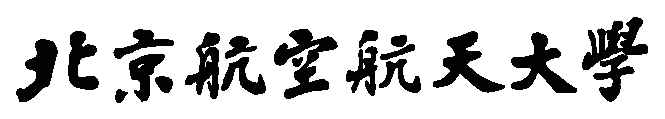
\includegraphics[width=.5\textwidth]{pic/logo-buaa}
  \caption{测试图片\\第二行题注}
  \label{fig:logo}
\end{figure}
\centerline{-----------$\uparrow$-----------Space Check-----------$\uparrow$-----------}

我们在这儿插入一行字;

我们在这儿再插入一行字;

我们在这儿插入一行字;

我们在这儿再插入一行字;

我们在这儿插入一行字;

我们在这儿再插入一行字;

我们在这儿插入一行字;

我们在这儿再插入一行字;

\section{数学环境}

\subsection{数学符号}

模板定义了一些正体(upright)的数学符号:
\begin{center}
  \begin{tabular}{rl}
    \toprule
    符号                 & 命令 \\
    \midrule
    常数$\eu$     & \verb|\eu| \\
    复数单位$\iu$ & \verb|\iu| \\
    微分符号$\diff$ & \verb|\diff| \\
    $\argmax$         & \verb|\argmax| \\
    $\argmin$         & \verb|\argmin| \\
    \bottomrule
  \end{tabular}
\end{center}

更多的例子:
\begin{equation}
\eu^{\iu\pi} + 1 = 0
\end{equation}
\begin{equation}
\frac{\diff^2u}{\diff t^2} = \int f(x) \diff x
\end{equation}
\begin{equation}
\argmin_x f(x)
\end{equation}

\subsection{定理、引理和证明}

\begin{definition}
  If the integral of function $f$ is measurable and non-negative, we define
  its (extended) \textbf{Lebesgue integral} by
  \begin{equation}
  \int f = \sup_g \int g,
  \end{equation}
  where the supremum is taken over all measurable functions $g$ such that
  $0 \leq g \leq f$, and where $g$ is bounded and supported on a set of
  finite measure.
\end{definition}

\begin{example}
  Simple examples of functions on $\mathbf{R}^d$ that are integrable
  (or non-integrable) are given by
  \begin{equation}
  f_a(x) =
  \begin{cases}
  |x|^{-a} & \text{if } |x| \leq 1,\\
  0 & \text{if } x > 1.
  \end{cases}
  \end{equation}
  \begin{equation}
  F_a(x) = \frac{1}{1 + |x|^a}, \qquad \text{all } x \in \mathbf{R}^d.
  \end{equation}
  Then $f_a$ is integrable exactly when $a < d$, while $F_a$ is integrable
  exactly when $a > d$.
\end{example}

\begin{lemma}[Fatou]
  Suppose $\{f_n\}$ is a sequence of measurable functions with $f_n \geq 0$.
  If $\lim_{n \to \infty} f_n(x) = f(x)$ for a.e. $x$, then
  \begin{equation}
  \int f \leq \liminf_{n \to \infty} \int f_n.
  \end{equation}
\end{lemma}

\begin{remark}
  We do not exclude the cases $\int f = \infty$,
  or $\liminf_{n \to \infty} f_n = \infty$.
\end{remark}

\begin{corollary}
  Suppose $f$ is a non-negative measurable function, and $\{f_n\}$ a sequence
  of non-negative measurable functions with
  $f_n(x) \leq f(x)$ and $f_n(x) \to f(x)$ for almost every $x$. Then
  \begin{equation}
  \lim_{n \to \infty} \int f_n = \int f.
  \end{equation}
\end{corollary}

\begin{proposition}
  Suppose $f$ is integrable on $\mathbf{R}^d$. Then for every $\epsilon > 0$:
  \begin{enumerate}
    \renewcommand{\theenumi}{\roman{enumi}}
    \item There exists a set of finite measure $B$ (a ball, for example) such that
    \begin{equation}
    \int_{B^c} |f| < \epsilon.
    \end{equation}
    \item There is a $\delta > 0$ such that
    \begin{equation}
    \int_E |f| < \epsilon \qquad \text{whenever } m(E) < \delta.
    \end{equation}
  \end{enumerate}
\end{proposition}

\begin{theorem}
  Suppose $\{f_n\}$ is a sequence of measurable functions such that
  $f_n(x) \to f(x)$ a.e. $x$, as $n$ tends to infinity.
  If $|f_n(x)| \leq g(x)$, where $g$ is integrable, then
  \begin{equation}
  \int |f_n - f| \to 0 \qquad \text{as } n \to \infty,
  \end{equation}
  and consequently
  \begin{equation}
  \int f_n \to \int f \qquad \text{as } n \to \infty.
  \end{equation}
\end{theorem}

\begin{proof}
  Trivial.
\end{proof}



\subsection{自定义}

\newtheorem*{axiomofchoice}{Axiom of choice}
\begin{axiomofchoice}
  Suppose $E$ is a set and ${E_\alpha}$ is a collection of
  non-empty subsets of $E$. Then there is a function $\alpha
  \mapsto x_\alpha$ (a ``choice function'') such that
  \begin{equation}
  x_\alpha \in E_\alpha,\qquad \text{for all }\alpha.
  \end{equation}
\end{axiomofchoice}

\newtheorem{observation}{Observation}[chapter]
\begin{observation}
  Suppose a partially ordered set $P$ has the property
  that every chain has an upper bound in $P$. Then the
  set $P$ contains at least one maximal element.
\end{observation}
\begin{proof}[A concise proof]
  Obvious.
\end{proof}

\newtheorem{observationvar2}[observation]{Observationvar2}
\begin{observationvar2}
  Suppose a partially ordered set $P$ has the property
  that every chain has an upper bound in $P$. Then the
  set $P$ contains at least one maximal element.
\end{observationvar2}
\begin{proof}[A concise proof]
  Obvious.
\end{proof}

我们在这儿插入一行字;

我们在这儿再插入一行字;

我们在这儿插入一行字;

我们在这儿再插入一行字;

我们在这儿插入一行字;

我们在这儿再插入一行字;

我们在这儿插入一行字;

我们在这儿再插入一行字;

我们在这儿插入一行字;

我们在这儿再插入一行字;

我们在这儿插入一行字;

我们在这儿再插入一行字;

我们在这儿插入一行字;

我们在这儿再插入一行字;

我们在这儿插入一行字;

我们在这儿再插入一行字;

我们在这儿插入一行字;

我们在这儿再插入一行字;